\chapter{Motor Current Test} \label{app:motorCurrentTest}
\textbf{Name: Group 630}\\
\textbf{Date: 02/05 - 2016}

\subsubsection{Purpose}
Check the assumption that the asked motor torque is the one that it gives in reality.

\subsubsection{Setup}
The Cubli is put in equilibrium at approximately \SI{0}{^{\circ}}. 
It is plugged to a computer from which the correct code can be sent, started and to which the data can later be retrieved, through USB over an Secure SHell (SSH) connection.

\subsubsection{List of Equipment}
\begin{table}[H]
\begin{tabular}{|p{10cm}|p{4cm}|}
\hline%------------------------------------------------------------------------------------
  \textbf{Instrument}                &  \textbf{Type} \\
\hline%------------------------------------------------------------------------------------
  Computer                           &  Asus A55V  \\
\hline%------------------------------------------------------------------------------------
\end{tabular}
\end{table}

\subsubsection{Procedure}

\begin{enumerate}
  \item Plug the power supply given with the Cubli setup to a \si{220}{V} power outlet.
  \item Wait until the blue LEDs on the Beaglebone Black start blinking slowly and connect the USB cable to the PC.
  \item Send the binary compiled program of the controller to the board.
  \item Connect to a distant terminal on the Beaglebone Black through SSH and launch the program.
  \item Let the program run.
  \item Stop the program (by pressing \textit{Q} and \textit{ENTER}).
  \item Retrieve the log file from the Cubli setup with the recorded data.
\end{enumerate}

\subsubsection{Results}
\begin{figure}[H]
	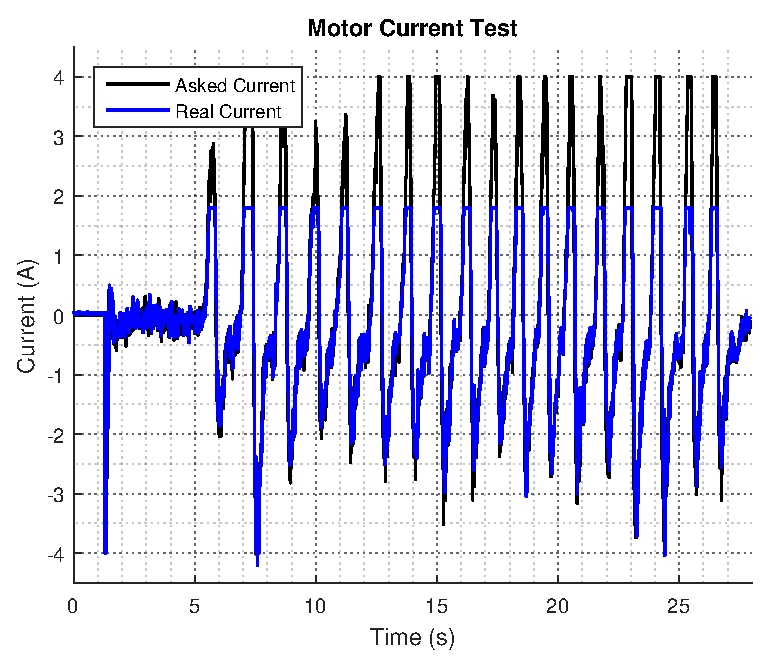
\includegraphics[scale=.65]{figures/motorCurrentTest}
	\centering
	\caption{}
\end{figure} \label{motorCurrentTest}

Note that the saturation on the blue curve is due to the AD converter, since the range for the value of current that the control board sends (-6,2 to 1,8A) goes from 4 to 0V, so any current above 1,8A will have saturation in the measurement.